\documentclass[11pt,a4paper]{article}
\usepackage[utf8]{inputenc}
\usepackage[T1]{fontenc}
\usepackage[spanish]{babel}
\usepackage{amsmath, amssymb, amsfonts}
\usepackage{graphicx}
\usepackage{geometry}
\geometry{a4paper, margin=2.5cm}
\usepackage{hyperref}
\hypersetup{
    colorlinks=true,
    linkcolor=blue,
    filecolor=magenta,
    urlcolor=cyan,
}
\usepackage{listings}
\usepackage{caption}
\usepackage{subcaption}
\usepackage{siunitx}
\usepackage{physics} % Para notación física

\title{Informe Parte B2: Integración de $e^{-x^2}$ por Monte Carlo}
\author{Física Computacional II - Grupo [Número/Nombre del Grupo]}
\date{\today}

\begin{document}
\maketitle
\tableofcontents
\newpage

\section{Objetivo}
El objetivo de esta parte del proyecto es calcular la integral definida de la función $f(x) = e^{-x^2}$ en el intervalo $[0, 1]$ utilizando el método de Monte Carlo por muestreo simple. Se analizará la convergencia del valor estimado de la integral y su error asociado en función del número de muestras $N$ utilizadas en la simulación.

La investigación teórica más amplia sobre el método de Monte Carlo y sus aplicaciones en física estadística se encuentra en el documento \texttt{../../documents/montecarlo\_fisica\_estadistica.tex}.

\section{Fundamento Teórico}
\subsection{Integración por Monte Carlo (Muestreo Simple)}
Dada una integral unidimensional de la forma:
\begin{equation}
    I = \int_a^b f(x) dx
\end{equation}
Podemos reescribirla como el producto del rango de integración y el valor esperado de $f(x)$ si $x$ es una variable aleatoria uniformemente distribuida en $[a,b]$:
\begin{equation}
    I = (b-a) \int_a^b f(x) p(x) dx = (b-a) \expval{f(X)}
\end{equation}
donde $p(x) = \frac{1}{b-a}$ para $x \in [a,b]$ y $0$ en otro caso.
El método de Monte Carlo estima este valor esperado promediando la función evaluada en $N$ puntos aleatorios $x_i$, generados uniformemente en $[a,b]$:
\begin{equation}
    I_N = (b-a) \frac{1}{N} \sum_{i=1}^N f(x_i)
\end{equation}
Por el Teorema del Límite Central, para $N$ grande, $I_N$ se aproxima a $I$.

\subsection{Estimación del Error}
El error estadístico (error estándar de la media) de la estimación $I_N$ está dado por:
\begin{equation}
    \text{Err}(I_N) = (b-a) \frac{\sigma_f}{\sqrt{N}}
\end{equation}
donde $\sigma_f^2$ es la varianza de la función $f(x)$ en el intervalo $[a,b]$:
\begin{equation}
    \sigma_f^2 = \expval{f^2(X)} - (\expval{f(X)})^2
\end{equation}
En la práctica, estimamos $\expval{f^2(X)}$ y $\expval{f(X)}$ a partir de las muestras:
\begin{align}
    \expval{f(X)} &\approx \frac{1}{N} \sum_{i=1}^N f(x_i) = \overline{f} \\
    \expval{f^2(X)} &\approx \frac{1}{N} \sum_{i=1}^N f^2(x_i) = \overline{f^2}
\end{align}
Entonces, el error estimado es:
\begin{equation}
    \text{Err}(I_N) \approx (b-a) \sqrt{\frac{\overline{f^2} - (\overline{f})^2}{N}}
\end{equation}
Este error disminuye como $N^{-1/2}$.

\subsection{La Integral Específica}
La integral a calcular es $I = \displaystyle\int_0^1 e^{-x^2}\,dx$.
Este valor es $\frac{\sqrt{\pi}}{2}\text{erf}(1)$, donde $\text{erf}(z) = \frac{2}{\sqrt{\pi}}\int_0^z e^{-t^2}dt$ es la función error.
El valor numérico de referencia es aproximadamente $0.7468241328$.

\section{Implementación}
Se desarrolló una clase \texttt{IntegradorMonteCarlo} en C++ que implementa el método de muestreo simple.
\begin{itemize}
    \item El constructor recibe la función a integrar (como \texttt{std::function<double(double)>}), los límites de integración y una semilla para el generador de números aleatorios (\texttt{std::mt19937}).
    \item El método \texttt{CalcularIntegralSimple} toma el número de muestras $N$ y devuelve el valor estimado de la integral y el error estándar calculado.
\end{itemize}
El programa principal (\texttt{main\_montecarlo\_integral.cpp}) utiliza esta clase para calcular la integral de $e^{-x^2}$ para un rango de valores de $N$ (desde $10^1$ hasta $10^7$) y guarda los resultados (N, valor estimado, error estimado, valor teórico, diferencia absoluta) en un archivo de datos para su posterior análisis y graficación.

\section{Resultados y Análisis}
\subsection{Convergencia del Valor de la Integral}
Se grafica el valor estimado de la integral en función del número de muestras $N$.
\begin{figure}[h!]
    \centering
    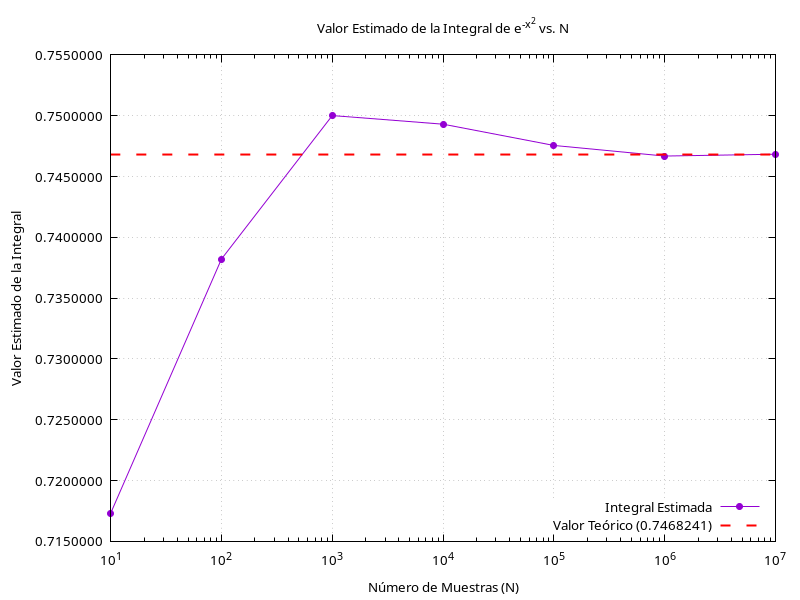
\includegraphics[width=0.8\textwidth]{../results/integral_mc_exp_neg_x2_valor_vs_N.png} % Ajustar nombre de archivo
    \caption{Valor estimado de $\int_0^1 e^{-x^2}dx$ en función del número de muestras $N$. La línea roja representa el valor teórico.}
    \label{fig:integral_valor}
\end{figure}
\textit{Discusión sobre cómo el valor estimado se acerca al valor teórico a medida que $N$ aumenta.}

\subsection{Convergencia del Error Estimado}
Se grafica el error estimado de la integral en función de $N$ en una escala log-log. Se espera una pendiente de $-1/2$.
\begin{figure}[h!]
    \centering
    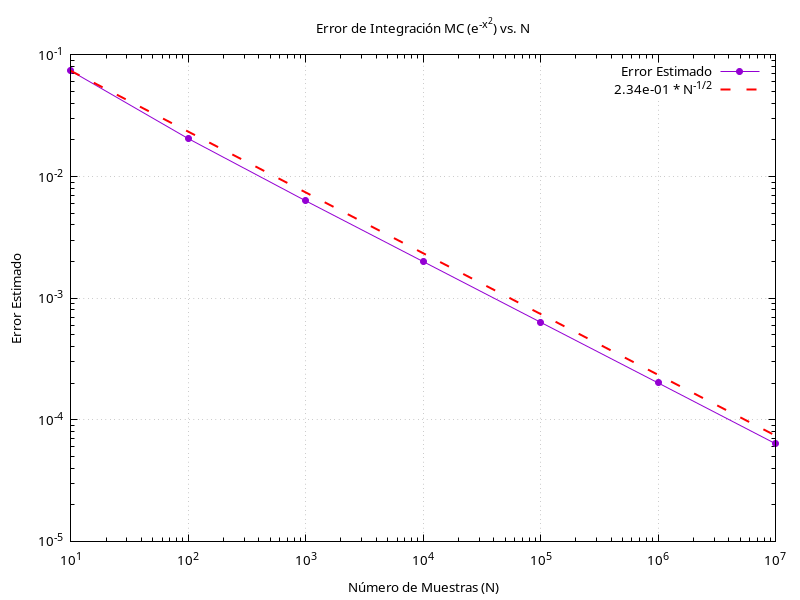
\includegraphics[width=0.8\textwidth]{../results/integral_mc_exp_neg_x2_error_vs_N.png} % Ajustar nombre de archivo
    \caption{Error estimado de la integral en función del número de muestras $N$ (escala log-log). La línea roja punteada muestra una referencia con pendiente $N^{-1/2}$.}
    \label{fig:integral_error}
\end{figure}
\textit{Análisis de la gráfica log-log del error. ¿Se observa la dependencia $N^{-1/2}$? Cálculo de la pendiente si es posible y comparación.}

\subsection{Diferencia Absoluta con el Valor Teórico}
También se analiza la diferencia absoluta entre el valor estimado y el valor teórico.
\begin{figure}[h!]
    \centering
    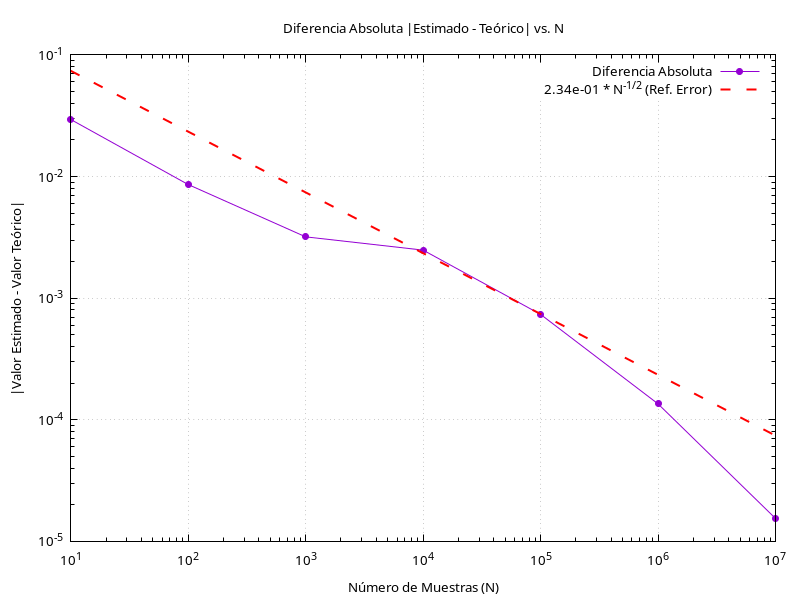
\includegraphics[width=0.8\textwidth]{../results/integral_mc_exp_neg_x2_diff_abs_vs_N.png} % Ajustar nombre de archivo
    \caption{Diferencia absoluta $|I_{estimado} - I_{teorico}|$ en función del número de muestras $N$ (escala log-log). La línea roja punteada es la referencia $N^{-1/2}$ del error estimado.}
    \label{fig:integral_diff_abs}
\end{figure}
\textit{Discusión: ¿La diferencia absoluta sigue la misma tendencia que el error estimado? ¿Hay fluctuaciones esperadas?}

\section{Conclusiones (Parte B2)}
Resumen de los resultados de la integración por Monte Carlo.
\begin{itemize}
    \item El método de Monte Carlo por muestreo simple converge al valor teórico de la integral.
    \item El error de la estimación disminuye con el número de muestras $N$ como $N^{-1/2}$, lo cual es característico de este método.
    \item Se ha implementado una clase reutilizable para la integración por Monte Carlo.
\end{itemize}

% \appendix
% \section{Código Fuente (Fragmentos)}
% \lstinputlisting[language=C++, caption=IntegradorMonteCarlo.h, basicstyle=\footnotesize\ttfamily]{../include/IntegradorMonteCarlo.h}

\end{document}
